
The background theory depth and breadth depends on the depth needed to understand your project in the different disciplines that your project crosses.  It is not a place to just write about everything you know that is vaguely connected to your project. The theory is here to help the reader that does not know the theoretical basis of your work so that he/she can gain sufficient understanding to understand your contributions. In particular, the theory section provides an opportunity to introduce terminology that can later be used without disturbing the text with a definition.  In some cases it will be more appropriate to have a separate section for different theory. However, watch that you don't end up with too short sections. Subsections may also be used to separate different background theory. 

When introducing techniques or results, always reference the source. Be careful to reference the original contributor of a technique and not just someone who happens to use the technique. For relevant results to your work, you would want to look particularly at newer results so that you have referenced the most up-to-date work in your area. If you don't have the source handy when writing, mark the test that a reference is needed and add it later. 

Web pages are not reliable sources --- they might be there one day and removed the next; and thus should be avoided, if possible. A verbal discussion is not a source and should not be referenced or described in the text.  

The bulk of citations in the report will appear in section~\ref{cit}. However, you will often need to introduce some terminology and key citations already in this chapter. 

You can cite a paper in the following manners: 

\begin{itemize}
\item when referring to authors:\\
 \citet{Bandara2019} stated something rather nice.
\item to cite indirectly: \\
 Papers should be written nicely \citep{Bandara2019}\\
or\\
In \cite{Bandara2019}, a less detailed template was presented.
\item To just cite the authors: \\
\citeauthor{Bandara2019} wrote a nice paper.
\item Or just the year: \citeyear{Bandara2019}.
\item You can even cite specific pages: \citet[p. 3]{Bandara2019}.
\end{itemize}

\vspace{0.5cm}

\noindent
{\bf Introducing figures:} \\

\begin{figure}[ht]
\begin{center}
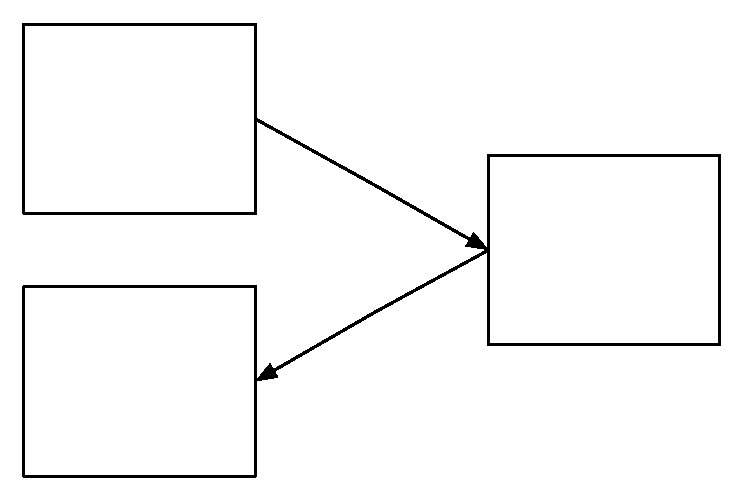
\includegraphics[width=0.5\columnwidth]{figs/figure1.pdf}
\caption[Boxes and arrows are nice]{Boxes and arrows are nice (adapted from \citet{Bandara2019})}
\label{fig:BoxesAndArrowsAreNice}
\end{center}
\end{figure}

Remember that when you borrow figures you should always credit the original author --- such as Figure \ref{fig:BoxesAndArrowsAreNice} (adapted from \citet{Bandara2019}). Also don't just put the figure in and leave it to the author to try to understand what the figure is. The figure should be put in to convey a message and you need to help the author to understand the message intended by explaining the figure in the text. 

\vspace{0.5cm}

\noindent
{\bf Introducing tables in the report: }\\

\begin{table}[htbp]
\begin{center}
\begin{tabular}{|c|c|c|c|c|}\hline\hline
This & is & a & nice & table\\\hline
This & is & a & nice & table\\\hline\hline
\end{tabular}
\caption{Example Table}
\end{center}
\label{tab:ExampleTable}
\end{table}%

As you can see from Table \ref{tab:ExampleTable}, tables are nice. However, again, you need to discuss the contents of the table in the text. You don't need to describe every entry but draw the authors attention to what is important for he/she to glean from the table. 
